\section{Résultats}

\paragraph*{Mesures}
L'approche critique a été réalisée en commencant à \(h_0 = 920.0 \pm 0.1\) mm. À chaque hauteur d'eau, le courant \(I\), ainsi que le nombre de neutrons \(N\) et le temps écoulé \(t\) ont été mesurés. Le taux de comptage \(C\) est alors déterminé avec \(C = N/t\). Les hauteurs où les mesures ont été réalisées ainsi que les valeurs mesurées sont reportées dans le \autoref{tab:mesures}.

\begin{table}[h]
    \centering
    \begin{tabular}{ |c||c|c|c|c|c| }
        \hline
        h [mm] & I [nA] & N & t [s] & C [\si{\per\second}] \\
        \hline\hline
        \(920.0 \pm 0.1\) & \(0.30 \pm 0.02\) & \(10006 \pm 1000\) & \(391.6 \pm 0.1\) & \(26 \pm 3\) \\
        \(930.0 \pm 0.1\) & \(0.42 \pm 0.02\) & \(10010 \pm 1000\) & \(279.8 \pm 0.1\) & \(36 \pm 4\) \\
        \(938.3 \pm 0.1\) & \(0.67 \pm 0.02\) & \(10002 \pm 1000\) & \(188.2 \pm 0.1\) & \(53 \pm 5\) \\
        \(943.1 \pm 0.1\) & \(1.1 \pm 0.2\) & \(10015 \pm 1000\) & \(126.9 \pm 0.1\) & \(79 \pm 8\) \\
        \hline
    \end{tabular}
    \caption{Hauteur d'eau dans le réacteur, courant, compte, temps de comptage et taux de comptage obtenus}
    \label{tab:mesures}
\end{table}

\paragraph{Estimations avec courant}
En accord avec la théorie, la hauteur d'eau est proportionnelle à l'inverse du courant. En utilisant la méthode décrite dans la démarche expérimentale, la hauteur critique \(h_c\) a été déterminée. Une estimation sur l'erreur est obtenue de manière graphique, comme décrit dans l'\autoref{sec:erreurs}. Les résultats sont présentés dans la \autoref{fig:hc_intensite}. Une hauteur critique entre 950 et 955 \si{\milli\meter} a alors été trouvée. Expérimentalement, l'opérateur a montré que la hauteur critique était \(h_c = 952.2 \pm 0.1\) mm.
\begin{figure}[H]
    \centering
    \begin{subfigure}{0.48\linewidth}
        \centering
        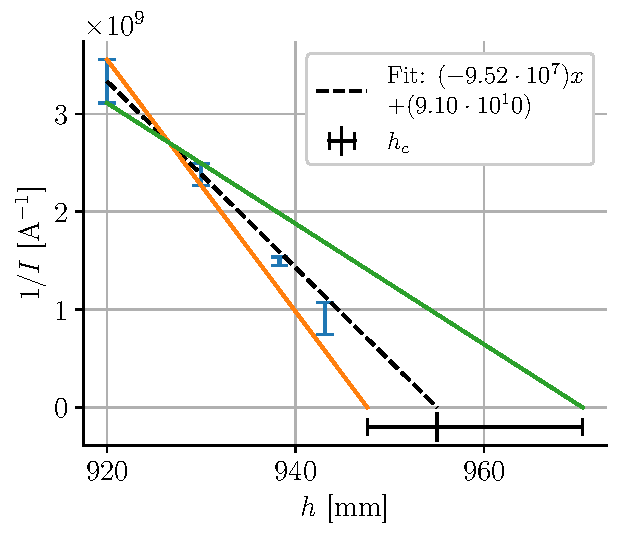
\includegraphics[width=\linewidth]{figures/h_I_pair12.pdf}
        \caption{}
        \label{fig:hc_I_12}
    \end{subfigure}
    \begin{subfigure}{0.48\linewidth}
        \centering
        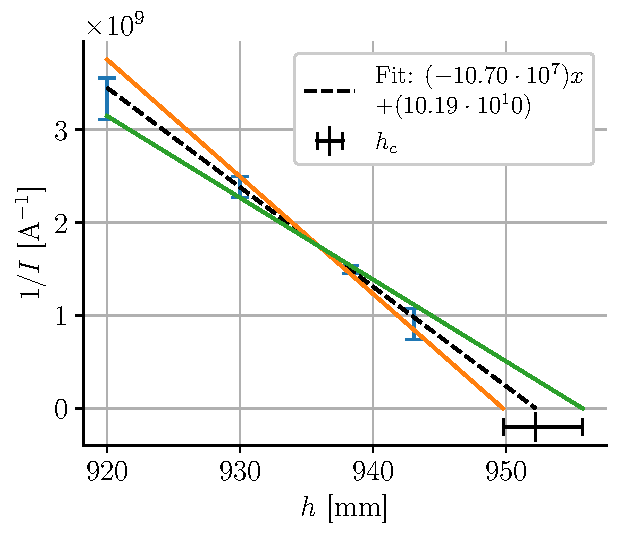
\includegraphics[width=\linewidth]{figures/h_I_pair23.pdf}
        \caption{}
        \label{fig:hc_I_23}
    \end{subfigure}
    \begin{subfigure}{0.48\linewidth}
        \centering
        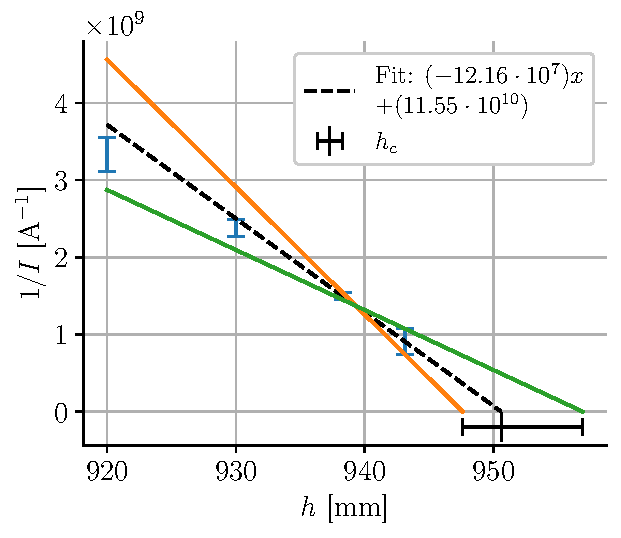
\includegraphics[width=\linewidth]{figures/h_I_pair34.pdf}
        \caption{}
        \label{fig:hc_I_34}
    \end{subfigure}
    \begin{subfigure}{0.48\linewidth}
        \centering
        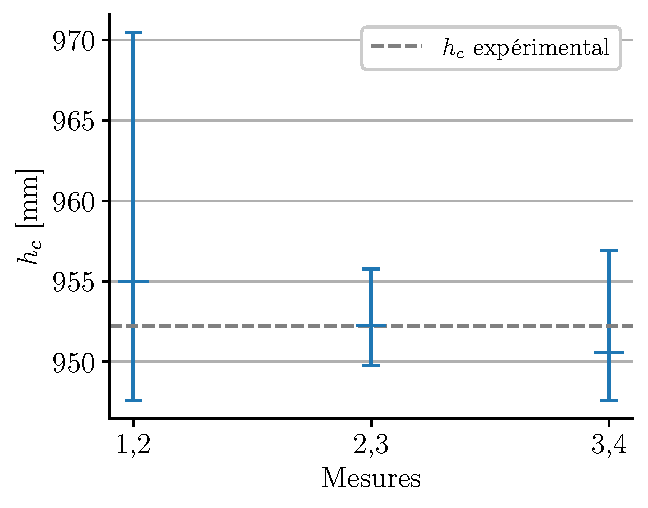
\includegraphics[width=\linewidth]{figures/hc_results_I.pdf}
        \caption{}
        \label{fig:hc_I}
    \end{subfigure}
    \caption{Estimations de \(h_c\) avec une régression linéaire en utilisant les mesures du courant $I$ (a) 1 et 2, (b) 2 et 3, (c) 3 et 4. En (d) les hauteurs critiques \(h_c\) trouvées, ainsi que l'estimation de l'erreur sur la valeur trouvée.}
    \label{fig:hc_intensite}
\end{figure}

\paragraph*{Estimations avec taux de comptage}
Pour l'estimation avec le nombre de neutrons détectés par seconde, la proportionnalité entre $1/C$ et $h$ a également été vérifiée expérimentalement. A l'aide de la même méthode que pour l'estimation avec le courant la hauteur critique $h_C$ a été déterminée et des erreurs sur ces résultats ont été obtenues de manière graphique. Ces résultats sont montrés en \autoref{fig:hc_compte}. Les hauteurs critiques trouvées ont donc été dans l'ordre des mesures: $h_{C,1,2} = 960 \pm 40$ \si{\milli \meter}, $h_{C,2,3} = 960 \pm 20$ \si{\milli \meter}, $h_{C,3,4} = 950 \pm 10$ \si{\milli \meter}. La comparaison de ces valeurs et de la hauteur de criticité expérimentale est faite en \autoref{fig:hc_C}
\begin{figure}[H]
    \centering
    \begin{subfigure}{0.48\linewidth}
        \centering
        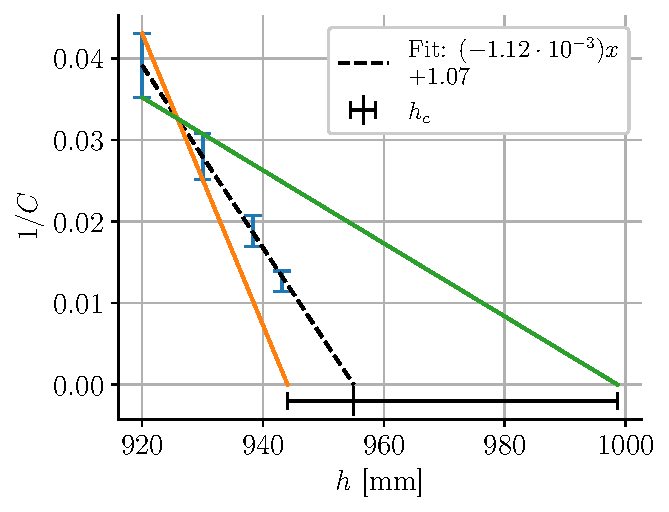
\includegraphics[width=\linewidth]{figures/h_C_pair12.pdf}
        \caption{}
        \label{fig:hc_C_12}
    \end{subfigure}
    \begin{subfigure}{0.48\linewidth}
        \centering
        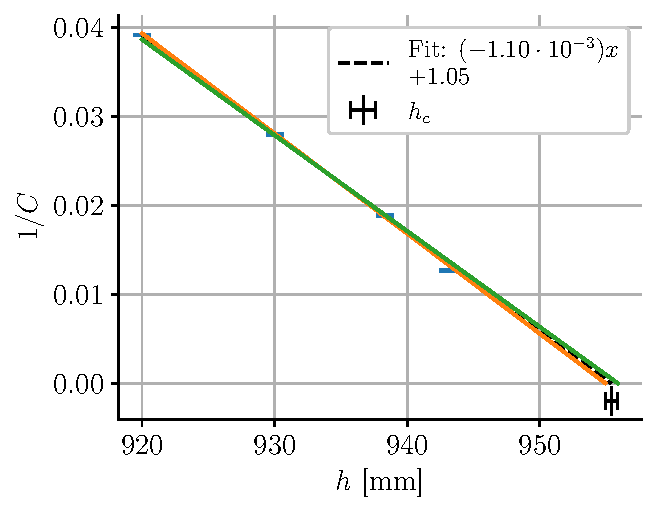
\includegraphics[width=\linewidth]{figures/h_C_pair23.pdf}
        \caption{}
        \label{fig:hc_C_23}
    \end{subfigure}
    \begin{subfigure}{0.48\linewidth}
        \centering
        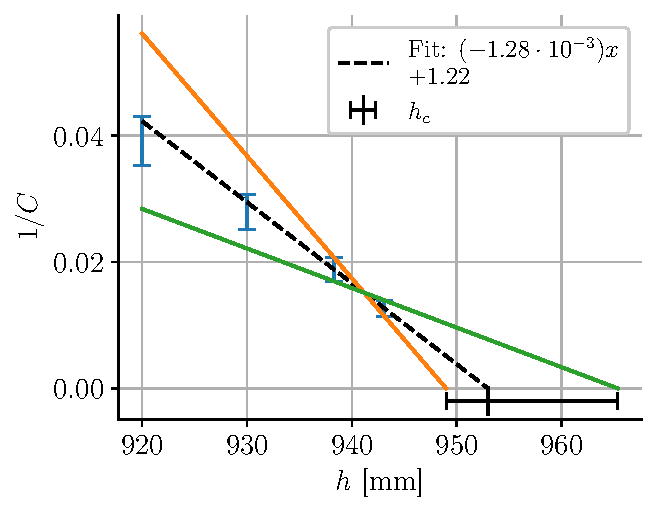
\includegraphics[width=\linewidth]{figures/h_C_pair34.pdf}
        \caption{}
        \label{fig:hc_C_34}
    \end{subfigure}
    \begin{subfigure}{0.48\linewidth}
        \centering
        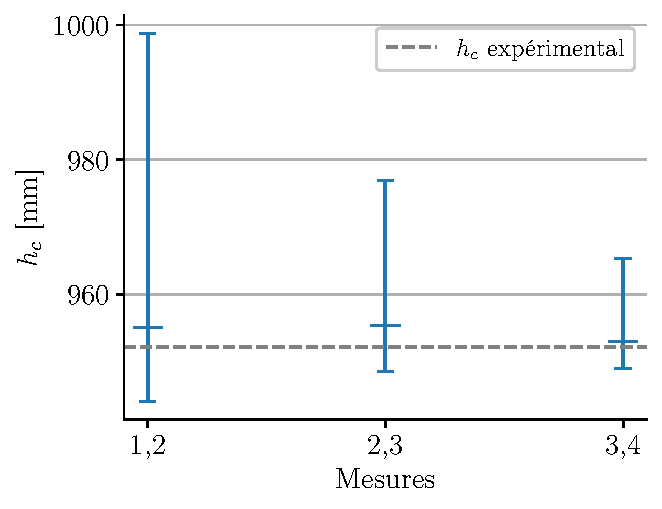
\includegraphics[width=\linewidth]{figures/hc_results_C.pdf}
        \caption{}
        \label{fig:hc_C}
    \end{subfigure}
    \caption{Estimations de \(h_c\) avec une régression linéaire en utilisant le nombre de neutrons par seconde $C$ mesurés (a) 1 et 2, (b) 2 et 3, (c) 3 et 4. En (d) les hauteurs critiques \(h_c\) trouvées, ainsi que l'estimation de l'erreur sur la valeur trouvée.}
    \label{fig:hc_compte}
\end{figure}